\section{CMDB}
Eine \acf{CMDB} ist ein aus dem \acf{ITIL} Umfeld stammendes Modell, um die IT-Infrastruktur eines Unternehmens abzubilden. Mit ihr kann auf Informationen zu Diensten und Konfigurationen zugegriffen werden.
\footcite[Vgl.][70\psq]{Olbrich_2008_ITIL}

Neben Hardware und Infrastruktur werden auch Dokumente wie Verträge, \acfp{SLA} oder Notfallpläne, sowie  Personen und Prozesse dort dokumentiert.
\footcite[Vgl.][253]{Sturm_2017_CMDB}


Die Komponenten einer \acs{CMDB} werden als \acfp{CI} bezeichnet. Ein \acf{CI} ist eine Einheit, die aus einem oder mehreren Objekten bestehen kann. Also z. B.~eine CPU, ein Kabel, ein kompletter Server, ein Netzwerksegment oder ein Cluster.
\footcite[Vgl.][70\psq]{Olbrich_2008_ITIL}

Zu den \acsp{CI} wird geplant, welchen Zweck diese erfüllen und in welchem Kontext sie eingesetzt werden (technisch und organisatorisch).
Es kann identifiziert werden, wer für das \acs{CI} zuständig ist und in welcher Version es vorliegt.
Sämtliche Änderungen an \acsp{CI} werden dokumentiert, wodurch eine vollständige Änderungshistorie über den gesamten Lebenszyklus entsteht.
\footcite[Vgl.][70\psq]{Olbrich_2008_ITIL}

Ein \acs{CI} kann verschiedene Eigenschaften bzw. Attribute besitzen und es können Verlinkungen zu anderen \acsp{CI} hergestellt werden, wodurch die Bildung einer Objekthierarchie möglich ist. Eine beispielhafte Anordnung ist in \autoref{fig:cih} zu sehen. \acsp{CI} werden außerdem in eine Kategorie eingeordnet und es kann ein Status zugewiesen werden.
\footcite[Vgl.][72\psqq]{Olbrich_2008_ITIL}

\begin{figure}[H]
  \centering
  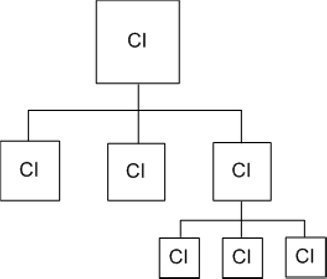
\includegraphics[width=0.3\textwidth]{Anhang/cih}
  \quelle[74]{Olbrich_2008_ITIL}
  \caption{Configuration Item Beziehungen}
\label{fig:cih}
\end{figure}


Neben rein hierarchischer Untergliederung sind auch andere Beziehungen zwischen \acsp{CI} möglich. Eine Übersicht mit Beispielen ist in \autoref{tab:bezci} zu sehen.\\
Durch die Verknüpfungen entsteht eine Übersicht, welche Systeme bei kritischen Ereignissen betroffen sind. Z. B.~welche Auswirkungen der Ausfall eines Switches hat.
\footcite[Vgl.][74\psq]{Olbrich_2008_ITIL}

\begin{table}[H]
\centering
\begin{tabularx}{0.8\textwidth}{l|X}
                            Beziehung & Beispiel \\\hline
                            X ist Teil von Y & eine CPU ist Teil eines Servers\\
                            X ist verbunden mit Y & ein Server ist mit einem Storagesystem verbunden \\
                            X benutzt Y & zwei Netzwerke benutzen eine VPN Verbindung \\
                            X ist eine Ausprägung von Y & gleicher Server, andere RAM Bestückung \\
\end{tabularx}
\quelleeigen[74]{Olbrich_2008_ITIL}
\caption{Beziehungen zwischen \aclp{CI}}
\label{tab:bezci}
\end{table}

%\begin{table}[H]
%\centering
%\begin{tabularx}{1\textwidth}{|l|X|}\hline
%                            Beziehung & Beispiel \\\hline\hline
%                            X ist Teil von Y & eine CPU ist Teil eines Servers\\\hline
%                            X ist verbunden mit Y & ein Server ist mit einem Storagesystem verbunden \\\hline
%                            X benutzt Y & zwei Netzwerke benutzen eine VPN Verbindung \\\hline
%                            X ist eine Ausprägung von Y & gleicher Server, andere RAM Bestückung \\\hline
%\end{tabularx}
%\quelleeigen[74]{Olbrich_2008_ITIL}
%\caption{Beziehungen zwischen \aclp{CI}}
%\label{tab:bezci}
%\end{table}


Jedes \acs{CI} durchläuft einen Lebenszyklus, der aus Beschaffung (Procurement), Betrieb (Operating) und Entsorgung (Disposal) besteht.
Die Beschaffung beinhaltet Bestellung und Lieferung. Sobald das \acs{CI} betriebsbereit ist, geht es in die Betriebsphase und wenn es ausgemustert wird, geht es in die Entsorgungsphase.\\
Je nach Phase können die \acsp{CI} verschiedene Zustände einnehmen. Diese können einen veränderbaren (V) oder finalen (F) Status haben. Eine Übersicht der Zustände pro Phase ist in \autoref{tab:statci} zu sehen.
\footcite[Vgl.][76\psq]{Olbrich_2008_ITIL}

\begin{table}[H]
\centering

\textit{Beschaffung}\\
\begin{tabularx}{.8\textwidth}{p{2cm}|c|X}
    Status      &  Art & Beschreibung                          \\\hline
    ordered     &  V & Bestellung wurde ausgelöst                 \\
    in progress &  V & Bestellvorgang wird bearbeitet             \\
    cancelled   &  F & Bestellung wurde storniert                 \\
    delivered   &  V & Ware wurde geliefert                       \\
    returned    &  F & Ware wurde zurückgesendet                  \\
\end{tabularx}

\bigskip\textit{Betrieb}\\
\begin{tabularx}{.8\textwidth}{p{2cm}|c|X}
    Status      &  Art & Beschreibung                          \\\hline
    active      &  V & CI ist im produktiven Einsatz              \\
    inactive    &  V & CI ist temporär nicht im Einsatz (Wartung) \\
    in store    &  V & CI ist im Lager                            \\
    planning    &  V & CI wird geplant                            \\
    test        &  V & CI wird getestet                           \\
\end{tabularx}

\bigskip\textit{Entsorgung}\\
\begin{tabularx}{.8\textwidth}{p{2cm}|c|X}
    Status      &  Art & Beschreibung                          \\\hline
    stolen      &  V & CI wurde gestohlen                         \\
    sold        &  F & CI wurde verkauft                          \\
    discarded   &  F & CI wurde ausgemustert                      \\
\end{tabularx}

\quelleeigen[77]{Olbrich_2008_ITIL}
\caption{Status von \aclp{CI}}
\label{tab:statci}
\end{table}


%\begin{table}[H]
%\centering
%
%\textit{Beschaffung}
%\begin{tabularx}{1\textwidth}{|p{2cm}|c|X|}\hline
%    Status      &  Art & Beschreibung                          \\\hline\hline
%    ordered     &  V & Bestellung wurde ausgelöst                 \\\hline
%    in progress &  V & Bestellvorgang wird bearbeitet             \\\hline
%    cancelled   &  F & Bestellung wurde storniert                 \\\hline
%    delivered   &  V & Ware wurde geliefert                       \\\hline
%    returned    &  F & Ware wurde zurückgesendet                  \\\hline
%\end{tabularx}
%
%\bigskip\textit{Betrieb}
%\begin{tabularx}{1\textwidth}{|p{2cm}|c|X|}\hline
%    Status      &  Art & Beschreibung                          \\\hline\hline
%    active      &  V & CI ist im produktiven Einsatz              \\\hline
%    inactive    &  V & CI ist temporär nicht im Einsatz (Wartung) \\\hline
%    in store    &  V & CI ist im Lager                            \\\hline
%    planning    &  V & CI wird geplant                            \\\hline
%    test        &  V & CI wird getestet                           \\\hline
%\end{tabularx}
%
%\bigskip\textit{Entsorgung}
%\begin{tabularx}{1\textwidth}{|p{2cm}|c|X|}\hline
%    Status      &  Art & Beschreibung                          \\\hline\hline
%    stolen      &  V & CI wurde gestohlen                         \\\hline
%    sold        &  F & CI wurde verkauft                          \\\hline
%    discarded   &  F & CI wurde ausgemustert                      \\\hline
%\end{tabularx}
%
%\quelleeigen[77]{Olbrich_2008_ITIL}
%\caption{Status von \aclp{CI}}
%\label{tab:statci}
%\end{table}


%\footcite[Vgl.][o. S.]{Drogseth_2015_CMDB}
%\footcite[Vgl.][o. S.]{Geissler_2018_CMDB}
%\footcite[Vgl.][o. S.]{Knittl_2010_CMDB}

% \footcite[Vgl.][o. S.]{itnovum_2013_cmdb}
% \footcite[Vgl.][o. S.]{Blokdijk_2008_CMDB}
